% easychair.tex,v 3.1 2011/12/30
%
% Select appropriate paper format in your document class as
% instructed by your conference organizers. Only withtimes
% and notimes can be used in proceedings created by EasyChair
%
% The available formats are 'letterpaper' and 'a4paper' with
% the former being the default if omitted as in the example
% below.
%
\documentclass[procedia]{easychair}
%\documentclass[debug]{easychair}
%\documentclass[verbose]{easychair}
%\documentclass[notimes]{easychair}
%\documentclass[withtimes]{easychair}
%\documentclass[a4paper]{easychair}
%\documentclass[letterpaper]{easychair}

% This provides the \BibTeX macro
\usepackage{doc}
\usepackage{makeidx}

% In order to save space or manage large tables or figures in a
% landcape-like text, you can use the rotating and pdflscape
% packages. Uncomment the desired from the below.
%
% \usepackage{rotating}
% \usepackage{pdflscape}

% If you plan on including some algorithm specification, we recommend
% the below package. Read more details on the custom options of the
% package documentation.
%
% \usepackage{algorithm2e}

% Some of our commands for this guide.
%
\newcommand{\easychair}{\textsf{easychair}}
\newcommand{\miktex}{MiK{\TeX}}
\newcommand{\texniccenter}{{\TeX}nicCenter}
\newcommand{\makefile}{\texttt{Makefile}}
\newcommand{\latexeditor}{LEd}

\def\procediaConference{International Conference on Computational Science (12-14 June, 2017)}

%\makeindex

%% Front Matter
%%
% Regular title as in the article class.
%
\title{Accelerating Parallel Multicriterial Optimization Methods 
Based on Intensive Using of Search Information}

% \titlerunning{} has to be set to either the main title or its shorter
% version for the running heads. When processed by
% EasyChair, this command is mandatory: a document without \titlerunning
% will be rejected by EasyChair

\titlerunning{Accelerating Parallel Multicriterial Optimization Methods}

% Authors are joined by \and. Their affiliations are given by \inst, which indexes into the list
% defined using \institute
%
\author{
    Gergel V.P.
\and
    Kozinov E.A.
}

% Institutes for affiliations are also joined by \and,
\institute{
  Lobachevsky State University of Nizhni Novgorod\\ 
	Nizhni Novgorod, Russia \\
  \email{gergel@unn.ru, evgeny.kozinov@itmm.unn.ru} 
 }
%  \authorrunning{} has to be set for the shorter version of the authors' names;
% otherwise a warning will be rendered in the running heads. When processed by
% EasyChair, this command is mandatory: a document without \authorrunning
% will be rejected by EasyChair

\authorrunning{Gergel and Kozinov}

\begin{document}

\maketitle

\keywords{decision making, multicriterial optimization, parallel computing, dimensionality reduction, criteria convolution, global optimization algorithms, computational complexity}

\begin{abstract}
  In the present paper, an efficient parallel method for solving complex multicriterial optimization problems, which the optimality criteria can be multiextremal, and the computing of the criteria values can require a large amount of computations in, is proposed. The proposed approach is based on the reduction of the multicriterial problems to the global optimization ones using the minimax convolution of the partial criteria, the dimensionality reduction with the use of the Peano space-filling curves, and the application of the efficient parallel information-statistical global optimization methods. The intensive use of the search information obtained in the course of computations is provided when conducting the computations. The results of the computational experiments demonstrated such an approach to allow reducing the computation costs of solving the multicriterial optimization problems essentially -- tens and hundreds times.
\end{abstract}

%\setcounter{tocdepth}{2}
%{\small
%\tableofcontents}

%\section{To mention}
%
%Processing in EasyChair - number of pages.
%
%Examples of how EasyChair processes papers. Caveats (replacement of EC
%class, errors).

%------------------------------------------------------------------------------
\section{Introduction}
\label{sect:1}

The multicriterial optimization (MCO) problem statements are used widely for modeling the complex decision making problems -- see, for example, the monographs \cite{c5,c7,c26,c27} and the reviews of the research and application results \cite{c8,c10,c20,c25}. 
Solving the MCO problems it should be taken into account that the partial optimality criteria are usually contradictory. As a result, solving the MCO problems is reduced to finding some compromised solutions, which the achievement of the best values with respect to the partial criteria is coordinated (the compromised solutions, which cannot be improved with respect to all partial criteria are usually called {\it nondominated}, {\it efficient} or {\it Pareto-optimal} solutions). At that, the understanding of an desired compromise may change in the course of computations that leads to the necessity to find several different efficient solutions -- in the limiting case, the whole set of the nondominated solutions (the Pareto domain).\par

The necessity to find several efficient solutions (or the whole Pareto domain) increases the computational complexity essentially. One must take into account also that the partial criteria can have a complex multiextremal form, and computing the criteria values can appear to be computation costly. In such conditions, finding even a single compromised solution requires considerable computations whereas computing several efficient solutions becomes a computational problem of the ultimate level of computational complexity. Overcoming this problem becomes possible with the use of huge computational capabilities of the supercomputing systems. And, besides, to provide the efficient computations, a full utilization of the search information obtained in the course of computations is necessary. \par

Further structure of the paper is as follows. In Section \ref{sect:2}, the multicriterial optimization problem statement is given. In Section \ref{sect:3}, the basics of the developed approach are presented: the reduction of the multicriterial problems to the global optimization ones by means of the minimax convolution of the partial criteria and the dimensionality reduction with the use of the Peano space-filling curves. In Section \ref{sect:4}, a parallel multicriterial global optimization algorithm utilizing the search information accumulated in the course of computations is presented. Section \ref{sect:5} involves the results of the numerical experiments. In Conclusions, the obtained results are discussed, and main directions of further investigations are outlined.


\section{Multicriterial Optimization Problem Statement}
\label{sect:2}
A multicriterial (multi-objective) optimization (MCO) problem can be defined as follows:
\begin{eqnarray} \label{eq:01}
f(y) = (f_1(y), f_2(y),\dots, f_s(y)) \to \min,  y \in D,
\end{eqnarray}
where $y = (y_1, y_2, \dots , y_N)$ is the vector of varied parameters, $N$ is the dimensionality of the multicriterial optimization problem being solved and $D$ is the search domain representing a $N$-dimensional hyperparallelepiped 
\begin{eqnarray*}
D  = \{ y \in R^N: a_i \leq y_i \leq b_i, 1 \leq i \leq N \}
\end{eqnarray*}
with given boundary vectors $a$ and $b$. Without loss of the generality, the partial criteria values in the problem (\ref{eq:01}) are supposed to be non-negative, and the decrease of these ones corresponds to the increase in the efficiency of the considered solutions $y \in D$.\par

As a solution of the MCO problem, any efficient solution (a {\it partial solution}) can be considered. In the general case, when solving a MCO problem, finding the whole set of nondominated solutions (the Pareto domain) $PD(f,D)$ ({\it a full solution of the MCO problem}) may be required. \par

Within the present paper, the MCO problems will be considered in application to the most complex decision making problems, which the partial criteria $f_i(y)$, $1 \leq i \leq s$ can be multiextremal, and obtaining the criteria values at the points of the search domain $y \in D$ can require a considerable amount of computations in. Let us suppose also the partial criteria $f_i(y)$, $1 \leq i \leq s$ to satisfy the Lipschitz condition
\begin{eqnarray} \label{eq:02}
|f_i(y') - f_i(y'')| \leq L_i \|y' - y''\|, y', y'' \in D, 1 \leq i \leq s. 
\end{eqnarray}

\section{Reduction Schemes for Multicriterial Problems}
\label{sect:3}
The proposed approach consists in the successive reduction of solving the MCO problems to solving a series of simpler optimization problems. In Subsection \ref{sect:3_1}, a method of the scalarization of the partial criteria, which reduces the MCO problem to a set of the global optimization ones is presented. In Subsection \ref{sect:3_2}, the dimensionality reduction with the use of the Peano space-filling curves that allows reducing the multidimensional optimization problems to the reduced one-dimensional global optimization ones is considered. \par

One can note the possibility to use a great number of efficient and widely used optimization methods for solving the MCO problems as an advantage of such an approach.


\subsection{Reducing the Multicriterial Problems to the Scalar Optimization Problems}
\label{sect:3_1}
A widely used approach for solving the MCO problems is the {\it scalarization approach}, which some methods of convolution of the set of partial criteria $f_i(y)$, $1 \leq i \leq s$ into a integrated scalar criterion $F(\lambda,y)$ are applied -- see, for example, \cite{c7,c8}. In the present paper, it is proposed to use a minimax convolution of the partial criteria in the form:
\begin{eqnarray} \label{eq:04}
F(\lambda,y) = \max_{1 \leq i \leq s}(\lambda_i f_i(y)), 
\end{eqnarray}
at given values of coefficients $\lambda_i$, $1 \leq i \leq s$, which the condition should be satisfied for
\begin{eqnarray*}
   \lambda \in  \Lambda \subset R^s:\sum_{i=1}^s{\lambda_i} = 1, \lambda_i \geq 0, 1 \leq i \leq s.
\end{eqnarray*}

The coefficients $\lambda_i$, $1 \leq i \leq s$ be understood as the indices of importance of the partial criteria -- the higher the value of the coefficient $\lambda_i$ for any particular partial criterion, the higher the contribution of this partial criterion into the integrated scalar criterion $F(\lambda,y)$. \par
 
It should be stressed that solving a MCO problem may require solving several problems (\ref{eq:04}) when changing the understanding of the importance of the partial criteria. The possibility to determine several efficient variants (or the whole Pareto domain) at reasonable computation costs becomes a key challenge in solving the complex multicriterial optimization problems.



\subsection{Reduction of the Multicriterial Problems to the One-dimensional Global Optimization Problems}
\label{sect:3_2}
In the general case, finding the numerical estimates of the globally-optimal extrema implies constructing a coverage of the search domain $D$ -- see, for example, \cite{c9,c11,c28,c35,c33,c42}. This fact complicates the computational schemes of the global optimization methods considerably since it implies a complex computational analysis of a large amount of multidimensional search information. As a result, many optimization algorithms utilize some methods of dimensionality reduction \cite{c13,c28,c32,c35,c33}.\par

Within the frames of the information-statistical approach, the {\it Peano curves} or {\it evolvents} $y(x)$ mapping the interval $[0,1]$ onto a $N$-dimensional hypercube $D$ unambiguously are used for the dimensionality reduction -- see, for example, \cite{c32,c35,c33}. As a result of such reduction, the initial multidimensional global optimization problem (\ref{eq:04}) is reduced to a one-dimensional one:
\begin{equation} \label{eq:05}
F(\lambda,y(x^*)) = \min_{x \in [0,1]} {F(\lambda,y(x))}.
\end{equation}

The considered dimensionality reduction scheme reduces a multidimensional problem with the Lipschitzian minimized function to a one-dimensional problem, which the corresponding functions satisfy the uniform H\"{o}lder condition (see \cite{c35,c33}) i. e.
\begin{eqnarray} \label{eq:06}
|F(\lambda,y(x')) - F(\lambda,y(x''))| \leq H |x' - x''|^{1/N}, x', x'' \in [0,1], 
\end{eqnarray}
where the constant $H$ is defined by the relation  $H = 4L \sqrt{N}$, $L$ is the Lipschitz constant from (\ref{eq:02}), and $N$ is the dimensionality of the optimization problem (\ref{eq:01}). \par

The algorithms for the numerical construction of the approximations of the Peano curves are presented in \cite{c35}.

\section{Parallel Computations for Global Optimization Problems}
\label{sect:4}
The approach presented in Section \ref{sect:3} allow reducing the solving of the MCO problem (\ref{eq:01}) to the solving a series of the reduced multiextremal problems (\ref{eq:05}). And, therefore, the problem of development of the methods for solving the MCO problems is resolved by the possibility of a wide application of the global optimization algorithms. Taking into account that the MCO problems can be computationally expensive the optimization methods should take advantage of the computational potential of high performance supercomputing systems. \par

In further description of the parallel computation methods, we will use a simpler notation of the reduced one-dimensional problems (\ref{eq:05}) as
\begin{eqnarray} \label{eq:07}
\varphi(x) = F(\lambda,y(x)): x \in [0,1]. 
\end{eqnarray}


\subsection{Parallel Algorithm of Multicriterial Global Optimization for the Computational Systems with Shared Memory}
\label{sect:4_1}
Within the framework of the proposed approach, the Parallel Multidimensional Algorithm of Global Search (PMAGS) \cite{c1,c15,c13,c16,c35,c33} is proposed to apply for solving every next reduced one-dimensional problem (\ref{eq:05}). The general computational scheme of this algorithm consists in the following.\par

Let $p$ be the number of parallel computational units (processors or cores) of a computational system with shared memory being used and let the minimized function values to be computed at any $p$ points of the interval $[0,1]$ (hereafter such computations will be called {\it trials}). Further, let $k$, $k>1$ parallel iterations of the global optimization be competed ($p$ trials are assumed to be performed within every parallel iteration). The choice of the trial points at the next $(k+1)^{th}$ parallel iteration is determined by the following rules.\par

{\it Rule 1.} Renumber the points from the set of all trial points executed earlier by the lower indices in the order of increasing coordinate value
\begin{equation} \label{eq:08}
0 = x_0 < x_1 < \dots < x_i < \dots < x_{kp} < x_{kp+1} = 1,
\end{equation}
the points $x_0$, $x_{kp+1}$ are introduced additionally for the convenience of further consideration, the minimized function values $z_0$, $z_{k+1}$ at these points remain undefined.

{\it Rule 2.} Compute the current estimate of the H\"{o}lder constant $H$ from (\ref{eq:06})
\begin{equation} \label{eq:09}
m = 
 \begin{cases}
   r M, & M > 0 \\
   1,   & M = 0
 \end{cases} ,
 M = \max_{1 \leq i \leq kp} {\frac{|z_i - z_{i-1}|} {\varrho_i} }
\end{equation}
as the relative differences of the minimized functions $\varphi(x)$ from (\ref{eq:07}) on the set of executed trial points $x_i$, $1 \leq i \leq kp$ from (\ref{eq:08}). Hereafter  $\varrho_i = (x_i - x_{i-1})^{1 / N}$, $1 \leq i \leq kp+1$. The constant $r$, $r>1$ is {\it the reliability parameter} of the algorithm.\par

{\it Rule 3.} Compute the {\it characteristics} $R(i)$ for each interval $(x_{i-1} ,x_i)$, $1 \leq i \leq kp+1$, where
\begin{equation} \label{eq:10}
\begin{matrix}
R(i) = \varrho_i + \frac{(z_i - z_{i-1})^2}{m^2 \varrho_i} - 2 \frac{(z_i + z_{i-1})}{m}, 1 \leq i \leq kp, \\
\\
R(i) = 2 \varrho_i - 4 \frac{z_{i}} {m} , i = 1, \\
\\
R(i) = 2 \varrho_i - 4 \frac{z_{i-1}} {m} , i = kp+1 \\
\end{matrix}
\end{equation}

{\it Rule 4.} Arrange the characteristics of the intervals obtained in (\ref{eq:10}) in the decreasing order 
\begin{equation} \label{eq:11}
  R(t_1) \geq R(t_2) \geq \dots \geq R(t_i) \geq \dots \geq R(t_{kp+1})
\end{equation}
and select $p$ intervals with the indices $t_j$, $1 \leq j \leq p$ having the maximal values of characteristics.\par

{\it Rule 5.} Execute new trials (the computations of the minimized function values) at the points $x^{kp+j}$ ,$1 \leq j \leq p$ located in the intervals with the maximal characteristics from (\ref{eq:11})
\begin{equation} \label{eq:12}
\begin{matrix}
x^{k+j} = \frac{x_{t_j} + x_{t_j-1}}{2} - sign(z_{t_j} - z_{t_j-1}) \frac{1}{2r} [\frac{|z_{t_j} - z_{t_j-1}|}{m}]^N, 1 < t_j < kp+1,\\
\\
x^{k+j} = \frac{x_{t_j} + x_{t_j-1}}{2}, t_j = 1 , t_j = kp + 1.
\end{matrix}
\end{equation}

The {\it termination condition}, according to which the trials are terminated, is defined by the condition 
\begin{equation} \label{eq:13}
\varrho_{t_j} < \varepsilon, 1 \leq j \leq p,
\end{equation}
which should be checked for all intervals from (\ref{eq:11}), which the scheduled trials are executed in. The parameter $\varepsilon > 0$ is the predefined {\it accuracy} of the problem solution. If the termination condition (\ref{eq:13}) is not satisfied, the iteration index $k$ is incremented by 1 (the number of the executed trials is incremented by $p$), and the next global optimization iteration is performed. \par

The characteristics $R(i)$, $1 \leq t \leq kp+1$ computed in (\ref{eq:10}) can be interpreted as some measures of importance of the intervals with respect to the location of the global minimum point in these ones. Then, the scheme of choosing the intervals for executing the next trials given by (\ref{eq:11})-(\ref{eq:12}) becomes clear -- the points for the next global optimization iteration are selected in the intervals, which the location of the global minimum point is the most probable in.\par

The conditions of convergence of the presented algorithm are considered, for example, in \cite{c35}. Thus, at an appropriate estimate of the H\"{o}lder constant ( $m > 2^{2-1/N}H$, $m$ is from (\ref{eq:09}) and $H$ is from (\ref{eq:06})) the algorithm converges to all existing global minimum points. 

\subsection{Accelerating the Computations Based on Intensive Using of Search Information}
\label{sect:4_2}
Solving the multicriterial optimization problems may require a considerable volume of computations. The reason of the computational complexity consists in the fact that in order to find several efficient solutions may require multiple solving of the global optimization problems (\ref{eq:04})-(\ref{eq:05}). The overcoming of this complexity can be provided by utilization of the search information obtained in the course of computations.\par

As a result of the scalarization of the partial criteria (\ref{eq:04}), the dimensionality reduction (\ref{eq:05}), and the necessity of the ordered representation (see Rule 1 of PMAGS), the search information can be represented as a {\it search state matrix} (SSM) 
\begin{equation} \label{eq:16}
A_k=\{(x_i,z_i,v_i )^T:0 \leq i \leq kp+1\}
\end{equation} 
where $x_i$, $0 \leq i \leq kp+1$ are the reduced points of the executed global optimization iterations, $z_i$, $1 \leq i \leq kp+1$ are the values of the scalar criterion of the current optimization problem (\ref{eq:05}), and $v_i$, $1 \leq i \leq kp+1$ are the calculated values of the partial criteria $f_i(y)$, $1 \leq i \leq s$. \par

Introducing SSM causes a crucial impact on an essential reduction of the computational complexity of solving the multicriterial optimization problems. The optimization methods can use SSM for the adaptive performing the next optimization iterations taking into account the results of previous computations. And, the most important, the availability of SSM allows transforming the results of all previous computations $z_i$, $1\leq i \leq kp$ stored in SSM to the values of the current optimization problem (\ref{eq:05}) for new values of the convolution coefficients $\lambda^{'}_j$, $1 \leq j \leq s$ i.e.
\begin{equation*}
z^{'}_i=\max_{1 \leq j \leq s}⁡(\lambda^{'}_j v_i(j)),1 \leq i \leq k,
\end{equation*}
without any time-consuming computations of the partial criteria values. And, therefore, all search information can be utilized in the continued computations. \par

The PMAGS algorithm expanded with the possibility to use the search information $A_k$ from (\ref{eq:16}) will be called hereafter Parallel Multidimensional Algorithm of Multicriterial Global Search (PMAMGS).

\section{Results of Computational Experiments}
\label{sect:5}
The computational experiments have been carried out on the Lobachevsky supercomputer at Lobachevsky State University of Nizhni Novgorod (the operating system -- CentOS 6.4, the supercomputer management system -- SLURM). A computational node included 2 Intel Sandy Bridge E5-2660 2.2 GHz processors, 64 Gb RAM. The CPUs had 8 cores (i. e. total 16 cores were available per a node). \par
 
Prior to describe the computational experiments, let us consider the results of comparing the proposed approach to a number of other multicriterial optimization algorithms presented in \cite{c14}. In the comparison, the bi-criteria two-dimensional problem proposed in \cite{c9}
\begin{equation}\label{eq:17}
f_1 (y)=(y_1-1) y_2^2+1, f_2 (y)=y_2, 0 \leq y_1,y_2 \leq 1,
\end{equation}
was used. The construction of a numerical approximation $PDA(f,D)$ of the Pareto domain $PD(f,D)$ was considered as the solution of the MCO problem. In order to evaluate the quality of the approximation, the completeness and the uniformity of coverage of the Pareto domain were compared using the following two indices \cite{c9,c42}:
\begin{itemize}
	\item 	The {\it hypervolume index} (HV) defined as the volume of the subdomain of the values of the vector criterion $f(y)$ dominated by the points of the Pareto domain approximation. The value of this index can be obtained as the total volume of the intersection of the hyperparallelepipeds, the vertices of which are the points of the Pareto domain approximation, and some reference point \^{f} ̂.This index features the completeness of an approximation of the Pareto domain (the larger the value, the more complete the coverage of the Pareto domain).
	\item 	The {\it distribution uniformity index} (DU) of the points from the Pareto domain approximation defined by the relations:
\begin{equation*}
\begin{matrix}
DI=\sum_{i=1}^p{(d_i-d)^2} , d=\dfrac{ \sum_{i=1}^p{d_i} }{p}, \\
d_i=\min {\varrho(y_i,y)}, y_i,y \in DPA, y_i \neq y, 1 \leq i \leq p,
\end{matrix}
\end{equation*}
where $p$ is the number of points in the Pareto domain approximation. This index features the uniformity of a coverage of the Pareto domain (the less the value, the more uniform the coverage of the Pareto domain).

\end{itemize}
Within the frames of this experiment, five multicriterial optimization algorithms have been compared:
\begin{itemize}
\item The Monte-Carlo (MC) method, in which the trial points were chosen randomly and uniformly within the search domain $D$,
\item The genetic algorithm SEMO from the PISA library \cite{c20,c42},
\item The Non-Uniform Coverage (NUC) method \cite{c20},
\item The Bi-objective Lipschitz Optimization (BLO) method proposed in \cite{c42},
\item The MAMGS (the serial version of PMAMGS) algorithm proposed in the present paper.
\end{itemize}
For the first three algorithms from the above list, the results of experiments from \cite{c20} have been used. For the BLO method, the results of experiments were presented in \cite{c42}. For MAMGS the following parameters were used: the reliability parameter $r = 3$ and the accuracy  $\varepsilon = 0.05$. Total 50 problems (\ref{eq:05}) with various convolution coefficients $\lambda$ distributed uniformly in $\Lambda$ from (\ref{eq:04}) have been solved by MAMGS.\par

The results of experiments from \cite{c14} are presented in Table \ref{tab:01}. The results have demonstrated that the MAMGS algorithm has a considerable advantage as compared to considered multicriterial optimization methods even when solving relatively simple MCO problems.

\begin{table}[t]
\centering
\caption{The results of computational experiments from \cite{c14} for the test problem (\ref{eq:17})}
\label{tab:01}
\begin{tabular}{cllll}
\hline
\textbf{Method} & \textbf{Iterations} & \textbf{PDA points} & \textbf{HV} & \textbf{DU} \\ \hline
MC              & 500                 & 67                  & 0.300       & 1.277       \\
SEMO            & 500                 & 104                 & 0.312       & 1.116       \\
NUC             & 515                 & 29                  & 0.306       & 0.210       \\
BLO             & 498                 & 68                  & 0.308       & 0.175       \\
MAMGS+          & 370                 & 100                 & 0.316       & 0.101       \\ \hline
\end{tabular}
\end{table}


In the executed series of experiments, the solving of bi-criteria two-dimensional MCO problems i.e. $N=2$, $s=2$ has been performed. The multiextremal functions defined below:
\begin{equation*}
\begin{matrix}
AB = \Big(\sum_{i=1}^7 \sum_{j=1}^7 [A_{ij} a_{ij}(y_1, y_2) + B_{ij} b_{ij}(y_1, y_2)]\Big)^2 \\
CD = \Big(\sum_{i=1}^7 \sum_{j=1}^7 [C_{ij} a_{ij}(y_1, y_2) - D_{ij} b_{ij}(y_1, y_2)]\Big)^2 \\ 
\phi(y_1, y_2) = - (AB + CD)^{1/2}
\end{matrix}
\end{equation*}
were used as the problem criteria. Here 
\begin{equation*}
\begin{matrix}
a_{ij}(y_1, y_2) = \sin(\pi i y_1) \sin(\pi j y_2), &
b_{ij}(y_1, y_2) = \cos(\pi i y_1) \cos(\pi j y_2)
\end{matrix}
\end{equation*}
are defined in the range $0 \leq y_1, y_2 \leq 1$, and the parameters  $-1\leq A_{ij},B_{ij},C_{ij},D_{ij} \leq 1$ are independent values distributed uniformly and randomly. The minimization of such functions arises, for example, in the problem of evaluation of the maximum strain (determined by the strength) in a thin plate at the transverse load. \par

In order to provide more justified conclusions on the efficiency of the developed approach, the solving of 100 multicriterial problems formed with the use of the multiextremal functions of the above problem family has been performed. For solving the optimization problems, the reliability parameter $r=2$ and the search accuracy $\varepsilon=0.001$ were used. In every experiment performed, the problem (\ref{eq:04}) has been solved for 50 various convolution coefficients with the use of the search information and without the one. The obtained results of experiments were averaged over the number of solved MCO problems (i. e. the results of experiments are presented below in average per one MCO problem, which the global search of the Pareto optimal solutions for 50 problems (\ref{eq:04}) has been performed within). As an example, an approximation of the Pareto domain obtained for a problem to be solved is shown in Figure \ref{fig:F1F2_gr}.

\begin{figure}
	\centering
	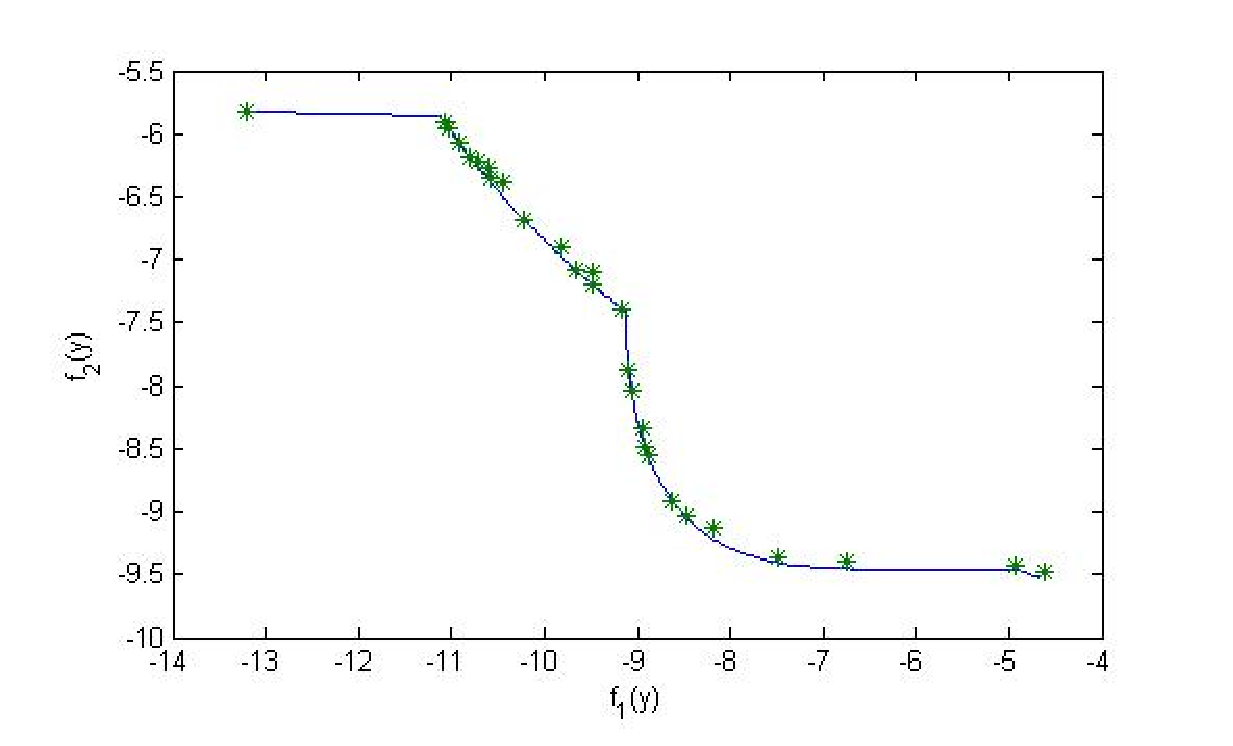
\includegraphics[width=0.45\textwidth]{F1F2_gr}
	\caption{Approximation of the Pareto domain for a MCO problem to be solved}
	\label{fig:F1F2_gr}
\end{figure}

The results of numerical experiments are presented in Table \ref{tab:02}.

\begin{table}[t]
\centering
\caption{The results of the series of experiments on solving the bi-criteria two-dimensional MCO problems}
\label{tab:02}
\begin{tabular}{cccccccc}
\hline
\multicolumn{1}{c}{\textbf{}}  &  & \multicolumn{2}{c}{\textbf{Iterations}}                                  &  & \multicolumn{3}{c}{\textbf{Speedup}}                                                                                   \\ \cline{3-4} \cline{6-8} 
\multicolumn{1}{c}{\textbf{p}} &  & \multicolumn{1}{c}{\textbf{PMAGS}} & \multicolumn{1}{c}{\textbf{PMAMGS}} &  & \multicolumn{1}{c}{\textbf{PMAGS}} & \multicolumn{1}{c}{\textbf{PMAMGS - 1}} & \multicolumn{1}{c}{\textbf{PMAMGS - 2}} \\ \cline{1-1} \cline{3-4} \cline{6-8}
1                              &  & 2                                  & 3                                   &  & 4                                  & 5                                       & 6                                       \\ \cline{1-1} \cline{3-4} \cline{6-8}
1                              &  & 17161,9                            & 1773,4                              &  & 1                                  & 1                                       & 9,7                                     \\
2                              &  & 9019,4                             & 1103,1                              &  & 1,9                                & 1,6                                     & 15,6                                    \\
5                              &  & 4117,2                             & 550,1                               &  & 4,2                                & 3,2                                     & 31,2                                    \\
10                             &  & 1801,7                             & 179,6                               &  & 9,5                                & 9,9                                     & 95,6                                    \\
25                             &  & 820,2                              & 77,5                                &  & 20,9                               & 22,9                                    & 221,4                                   \\ \hline
\end{tabular}
\end{table}

To explain the presented results, let us remind that PMAGS is a parallel algorithm without the use of the search information while PMAMGS uses the search information intensively. \par

The results of experiments demonstrate an essential reduction of the amount of computations by means of the use of the search information obtained in the course of the global optimization. Even for the serial algorithm without any use of the parallel computations, this reduction reaches more than 9 times (Column 6). In order to account for this result, two variants of obtained speedup are given in Table \ref{tab:02}: one relative to the serial algorithm utilizing the search information (Speedup 1, Column 5) and another one relative to the initial serial algorithm (Speedup 2, Column 6). As follows from the presented data, the speedup of the parallel computations with the use of the search information was 22.9 when using 25 computational cores. One should note a considerable increase of the speedup of the parallel computations relative to the initial algorithm without the use of the search information -- the speedup was 221.4 for 25 computational cores. In addition, the obtained results are presented also in the visual graphical form in Figure \ref{fig:res_exp}.

\begin{figure}
	\centering
	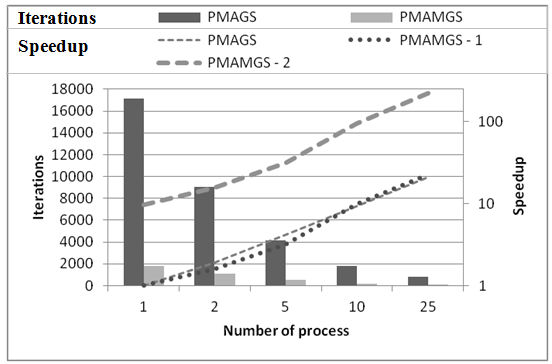
\includegraphics[width=0.45\textwidth]{res_exp}
	\caption{Diagrams for demonstrating the results of the numerical experiments}
	\label{fig:res_exp}
\end{figure}

In Figure \ref{fig:res_exp}, the bar chart demonstrates the number of parallel iterations executed by the methods (columns 2 and 3 in Table 2), the corresponding numbers are shown on the left axis. The line plots present the speedups of parallel computations (columns 5 and 6 in Table 2), the corresponding scale is shown on the right axis.

\section{Conclusions}
\label{sect:6}
In the present paper, an efficient parallel method for solving complex multicriterial optimization problems, which the criteria of optimality can be multiextremal, and the computing of the criteria values can require a large volume of computations in, has been proposed. The basis of the proposed approach consists in reduction of the multicriterial problems to the global optimization ones by means of the minimax convolution of the partial criteria, the dimensionality reduction with the use of the Peano space-filling curves, and the application of the efficient information-statistical global optimization methods. \par

The key aspect of the developed approach consists in the overcoming of large computations costs of the global optimization of the set of efficient solutions when solving the multicriterial optimization problems. A considerable increase of the efficiency and essential reduction of the amount of computations are provided by means of intensive using of the search information obtained in the course of computations. Within the framework of developed approach, a method for transforming all available search information to the values of current scalar problem of global optimization being solved have been proposed. The search information is used by the parallel optimization methods for the adaptive planning of the performed global optimization iterations. The results of the computational experiments demonstrated such an approach to allow reducing the computational costs of solving the multicriterial optimization problems essentially -- by tens and hundreds times. \par

In conclusion, one can note that the developed approach is a promising one and requires further investigations. First of all, it is necessary to continue carrying out the computational experiments on solving the multicriterial optimization problems with a large number of partial criteria of efficiency and for a greater dimensionality of the optimization problems being solved. It is necessary also to estimate the possibility to organize the parallel computations with the use of a greater number (hundreds and thousands) of processors in the high performance computational systems with the distributed memory.


\section{Acknowledgements}
\label{sect:7}

This work has been supported by Russian Science Foundation, project No 16-11-10150 ''Novel efficient methods and software tools for time-consuming decision making problems using superior-performance supercomputers.''
%------------------------------------------------------------------------------
% Refs:
%
\label{sect:bib}
\bibliographystyle{plain}
%\bibliographystyle{alpha}
%\bibliographystyle{unsrt}
%\bibliographystyle{abbrv}
\bibliography{iccs_2017}

%------------------------------------------------------------------------------
\end{document}

% EOF
